% This LaTeX was auto-generated from MATLAB code.
% To make changes, update the MATLAB code and export to LaTeX again.

\documentclass{article}

\usepackage[utf8]{inputenc}
\usepackage[T1]{fontenc}
\usepackage{lmodern}
\usepackage{graphicx}
\usepackage{color}
\usepackage{hyperref}
\usepackage{amsmath}
\usepackage{amsfonts}
\usepackage{epstopdf}
\usepackage[table]{xcolor}
\usepackage{matlab}

\sloppy
\epstopdfsetup{outdir=./}
\graphicspath{ {./week5_images/} }

\begin{document}
\begin{center}
\textbf{Ch3: Generalized inverse, individual activity}\\
\end{center}





$\textbf {1 (a)}$\\
\begin{align*}
	G^TG& = (U S V^T)^T (U S V^T)\\
	 &= (V S^T U^T) (U S V^T)\\
	  &= V S U^T US V^T\\
	  &= V S I S V^T\\
	  &= V S ^2 V ^T\\
	\end{align*}

$\textbf {1 (b)}$\\
\begin{center}
\includegraphics[width=\maxwidth{56.196688409433015em}]{1.jpg}
\end{center}

\begin{center}
\includegraphics[width=\maxwidth{56.196688409433015em}]{2.jpg}
\end{center}%\begin{align*}
	%G^TG& = (U_p S_p V_p^T)^T (U_p S_p V_p^T)\\
	%&= (V_pS_p^TU_p^T) (U_p S_p V_p^T)\\
%	&= V_pS_p U_p^T U_p S_p V_p^T\\
%	&= V_pS_p I_p S_p V_p^T\\
%	&= V_pS_p ^2 V_p^T\\
%\end{align*}
\begin{center}
\includegraphics[width=\maxwidth{56.196688409433015em}]{3.jpg}
\end{center}



$\textbf {1(c)}$\\
for $m>n$ and p=n , we have;

\begin{align*}
		G^{\dagger}&=  V_p S_p^{-1} U_p^	T\\
		&=  V_p S_p^{-2}V_p^TV_pS_p U_p^T\\
	\Rightarrow m_{\dagger} = G^{\dagger} d
	&=  V_p S_p^{-2}V_p^TV_pS_p U_p^T d\\
	& = V_p S_p^{-2}V_p^T G^T d
\end{align*}
But 
\begin{align*}
		(G^TG)^{-1}&= (V_pS_pU_p^TU_p S_p V_p^T)^{-1}\\
		&= V_pS_p^{-2} V_p^T
\end{align*}

\begin{align*}
		\Rightarrow  m_{\dagger} &= (G^TG)^{-1 }  G^T d
\end{align*}

Which is similar to the least squares estimates and hence $G^{\dagger} = (G^TG)^{-1 } G^T$ \\




$\textbf 2$\\

To show that $G^{\dagger}$ satisfies the four properties given below, we  used other properties  such as;  $U_p^T U_p = I_p $, $V_p^T V_p = I_p$ and $S_p  S_p^{-1}=S_p^{-1}S_p = I_p$  \\
 $\textbf{(a)}$
\begin{align*}
		GG^{\dagger}G& = (U_p S_p V_p^T V_p S_p^{-1} U_p^T)U_p S_p V_p^T\\
		&= (U_p S_p I_p S_p^{-1} U_p^T)U_p S_p V_p^T\\
		&= (U_p S_p  S_p^{-1} U_p^T)U_p S_p V_p^T\\
		&= U_p I_p  U_p^TU_p S_p V_p^T\\
		&= U_p S_p V_p^T\\
		&=G
	\end{align*}
	$\textbf{(b)}$
\begin{align*}
	G^{\dagger}GG^{\dagger}& = (V_p S_p^{-1} U_p^TU_p S_p V_p^T )V_p S_p^{-1} U_p^T\\
	&=  (V_p S_p^{-1} I_p S_p V_p^T )V_p S_p^{-1} U_p^T\\
	&=  (V_p S_p^{-1}S_p V_p^T )V_p S_p^{-1} U_p^T\\
	&=  V_p I_p V_p^T V_p S_p^{-1} U_p^T\\
	&=  V_p S_p^{-1} U_p^T\\
	&= G^{\dagger}
	\end{align*}	
	$\textbf{(c)}$
		\begin{align*}
		(GG^{\dagger})^T &=  (U_p S_p V_p^TV_p S_p^{-1} U_p^T)^T\\
		&=(U_p S_p  S_p^{-1} U_p^T)^T\\
		&=(U_p  U_p^T)^T \\
		&=U_p  U_p^T\\
		&= U_p S_p S_p^{-1}U_p^T\\
		&= U_p S_p V_p^T V_p  S_p^{-1}U_p^T\\
		&= (U_p S_p V_p^T )(V_p  S_p^{-1}U_p^T)\\
		&= GG^{\dagger}
		\end{align*}	
	$\textbf{(d)}$
\begin{align*}
	(G^{\dagger}G)^T &= (V_p S_p^{-1} U_p^TU_p S_p V_p^T)^T \\
	&= (V_p S_p^{-1}  S_p V_p^T)^T \\
	&= (V_p V_p^T)^T \\
	&=V_p V_p^T \\
	&= V_p S_p^{-1}  S_p  V_p^T\\
	&= V_p S_p^{-1}  U_p^TU_p S_p  V_p^T\\
	&=( V_p S_p^{-1}  U_p^T)(U_p S_p  V_p^T)\\
	&=G^{\dagger}G
\end{align*}	









3.(a) \\
\begin{align*}
m_{dagger} = 10^{-5} \times
\begin{bmatrix}
 -0.0369\\
   -0.8697\\
    0.1399\\
    0.0303\\
   -0.6702\\
    0.2732\\
    0.9732\\
    0.2066\\
    0.3536 \end{bmatrix}~~~~~~~m_{backslash} = 10^{-4} \times
\begin{bmatrix}
    -0.0070\\
   -0.0696\\
         0\\
   -0.0143\\
   -0.0637\\
    0.0413\\
    0.1180\\
         0\\
    0.0354\\
 \end{bmatrix}\end{align*}



\begin{center}
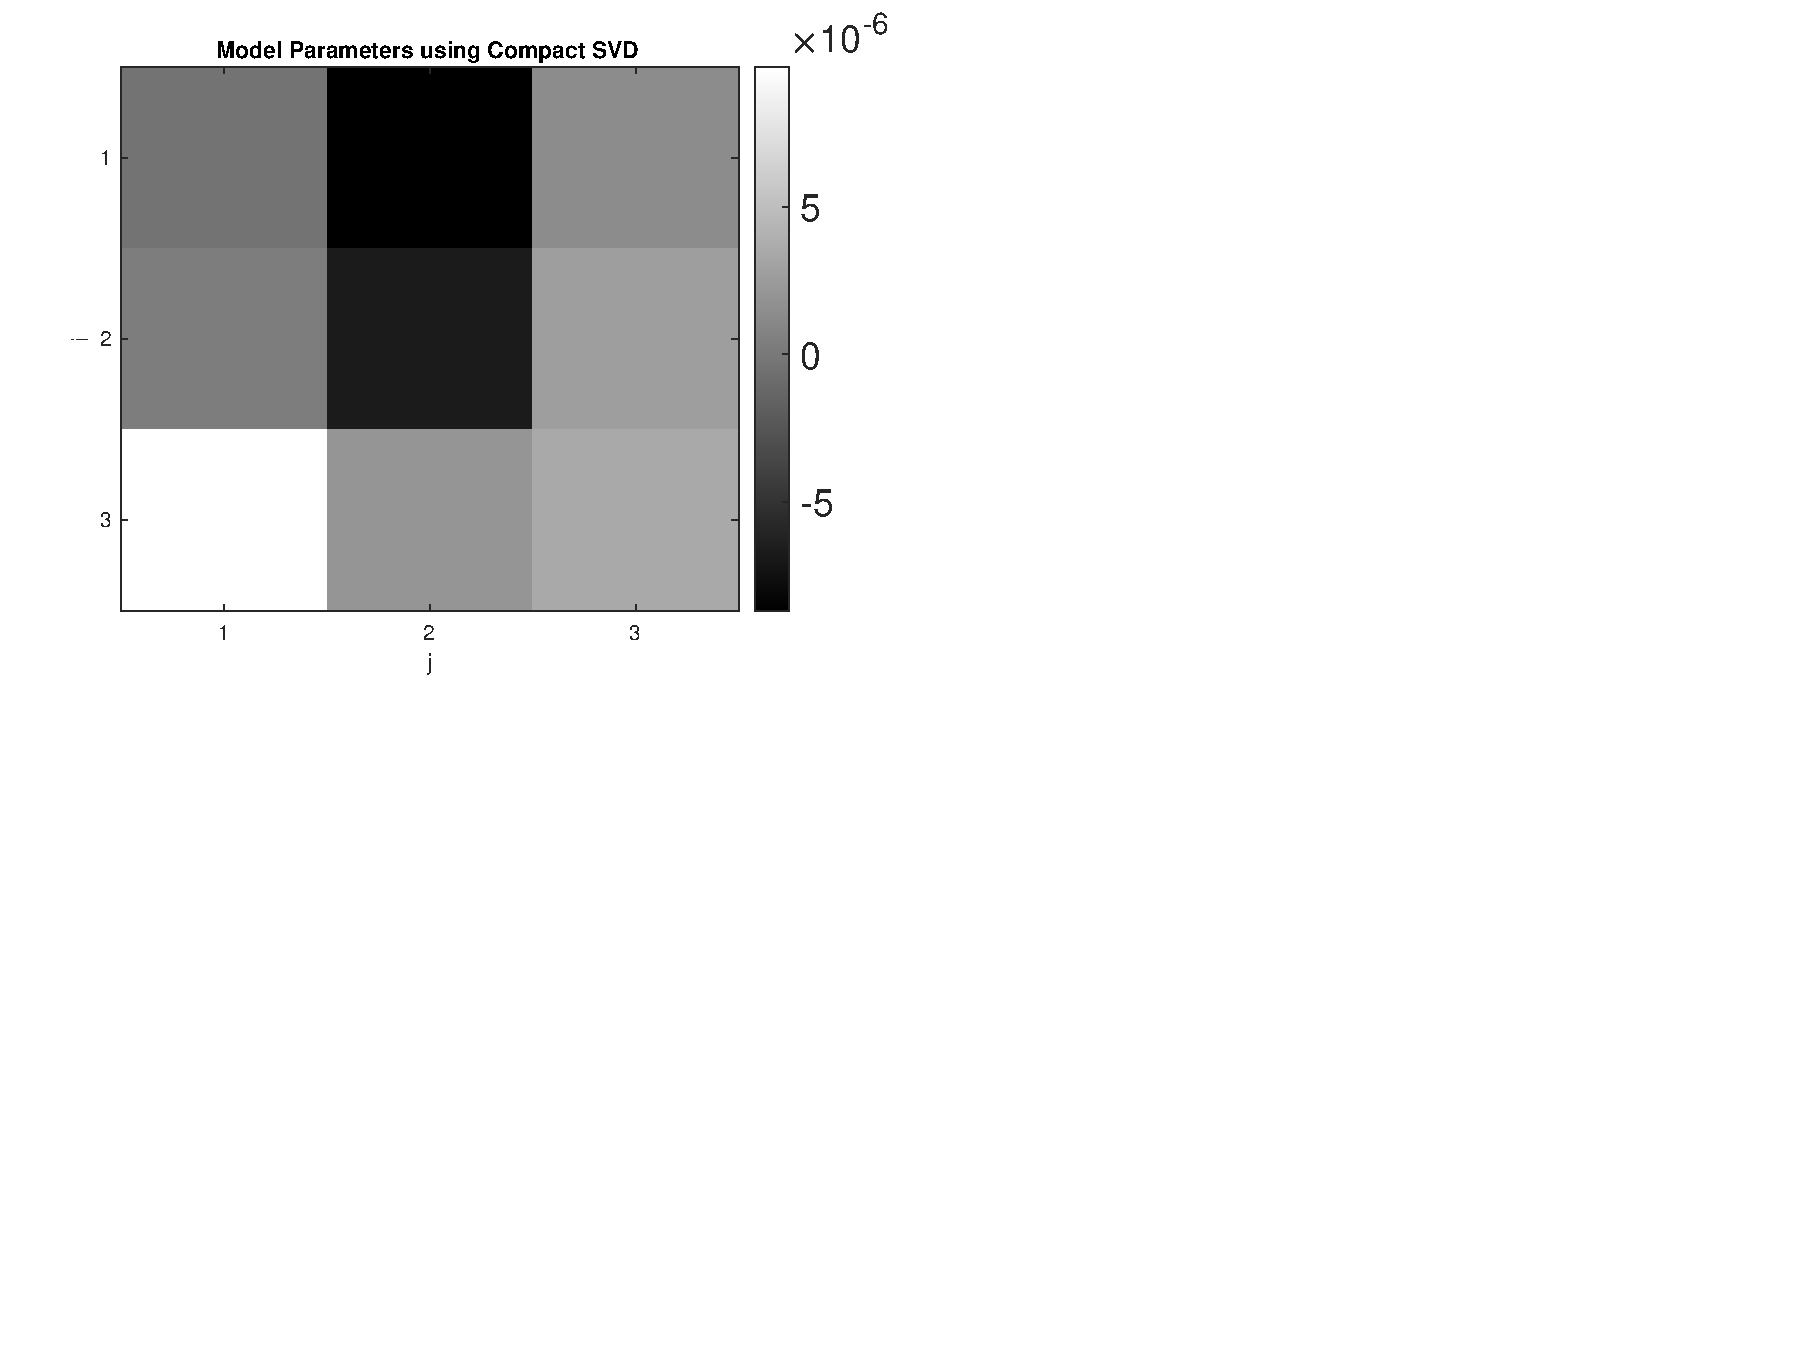
\includegraphics[width=\maxwidth{56.196688409433015em}]{figure_0.eps}
\end{center}

\begin{center}
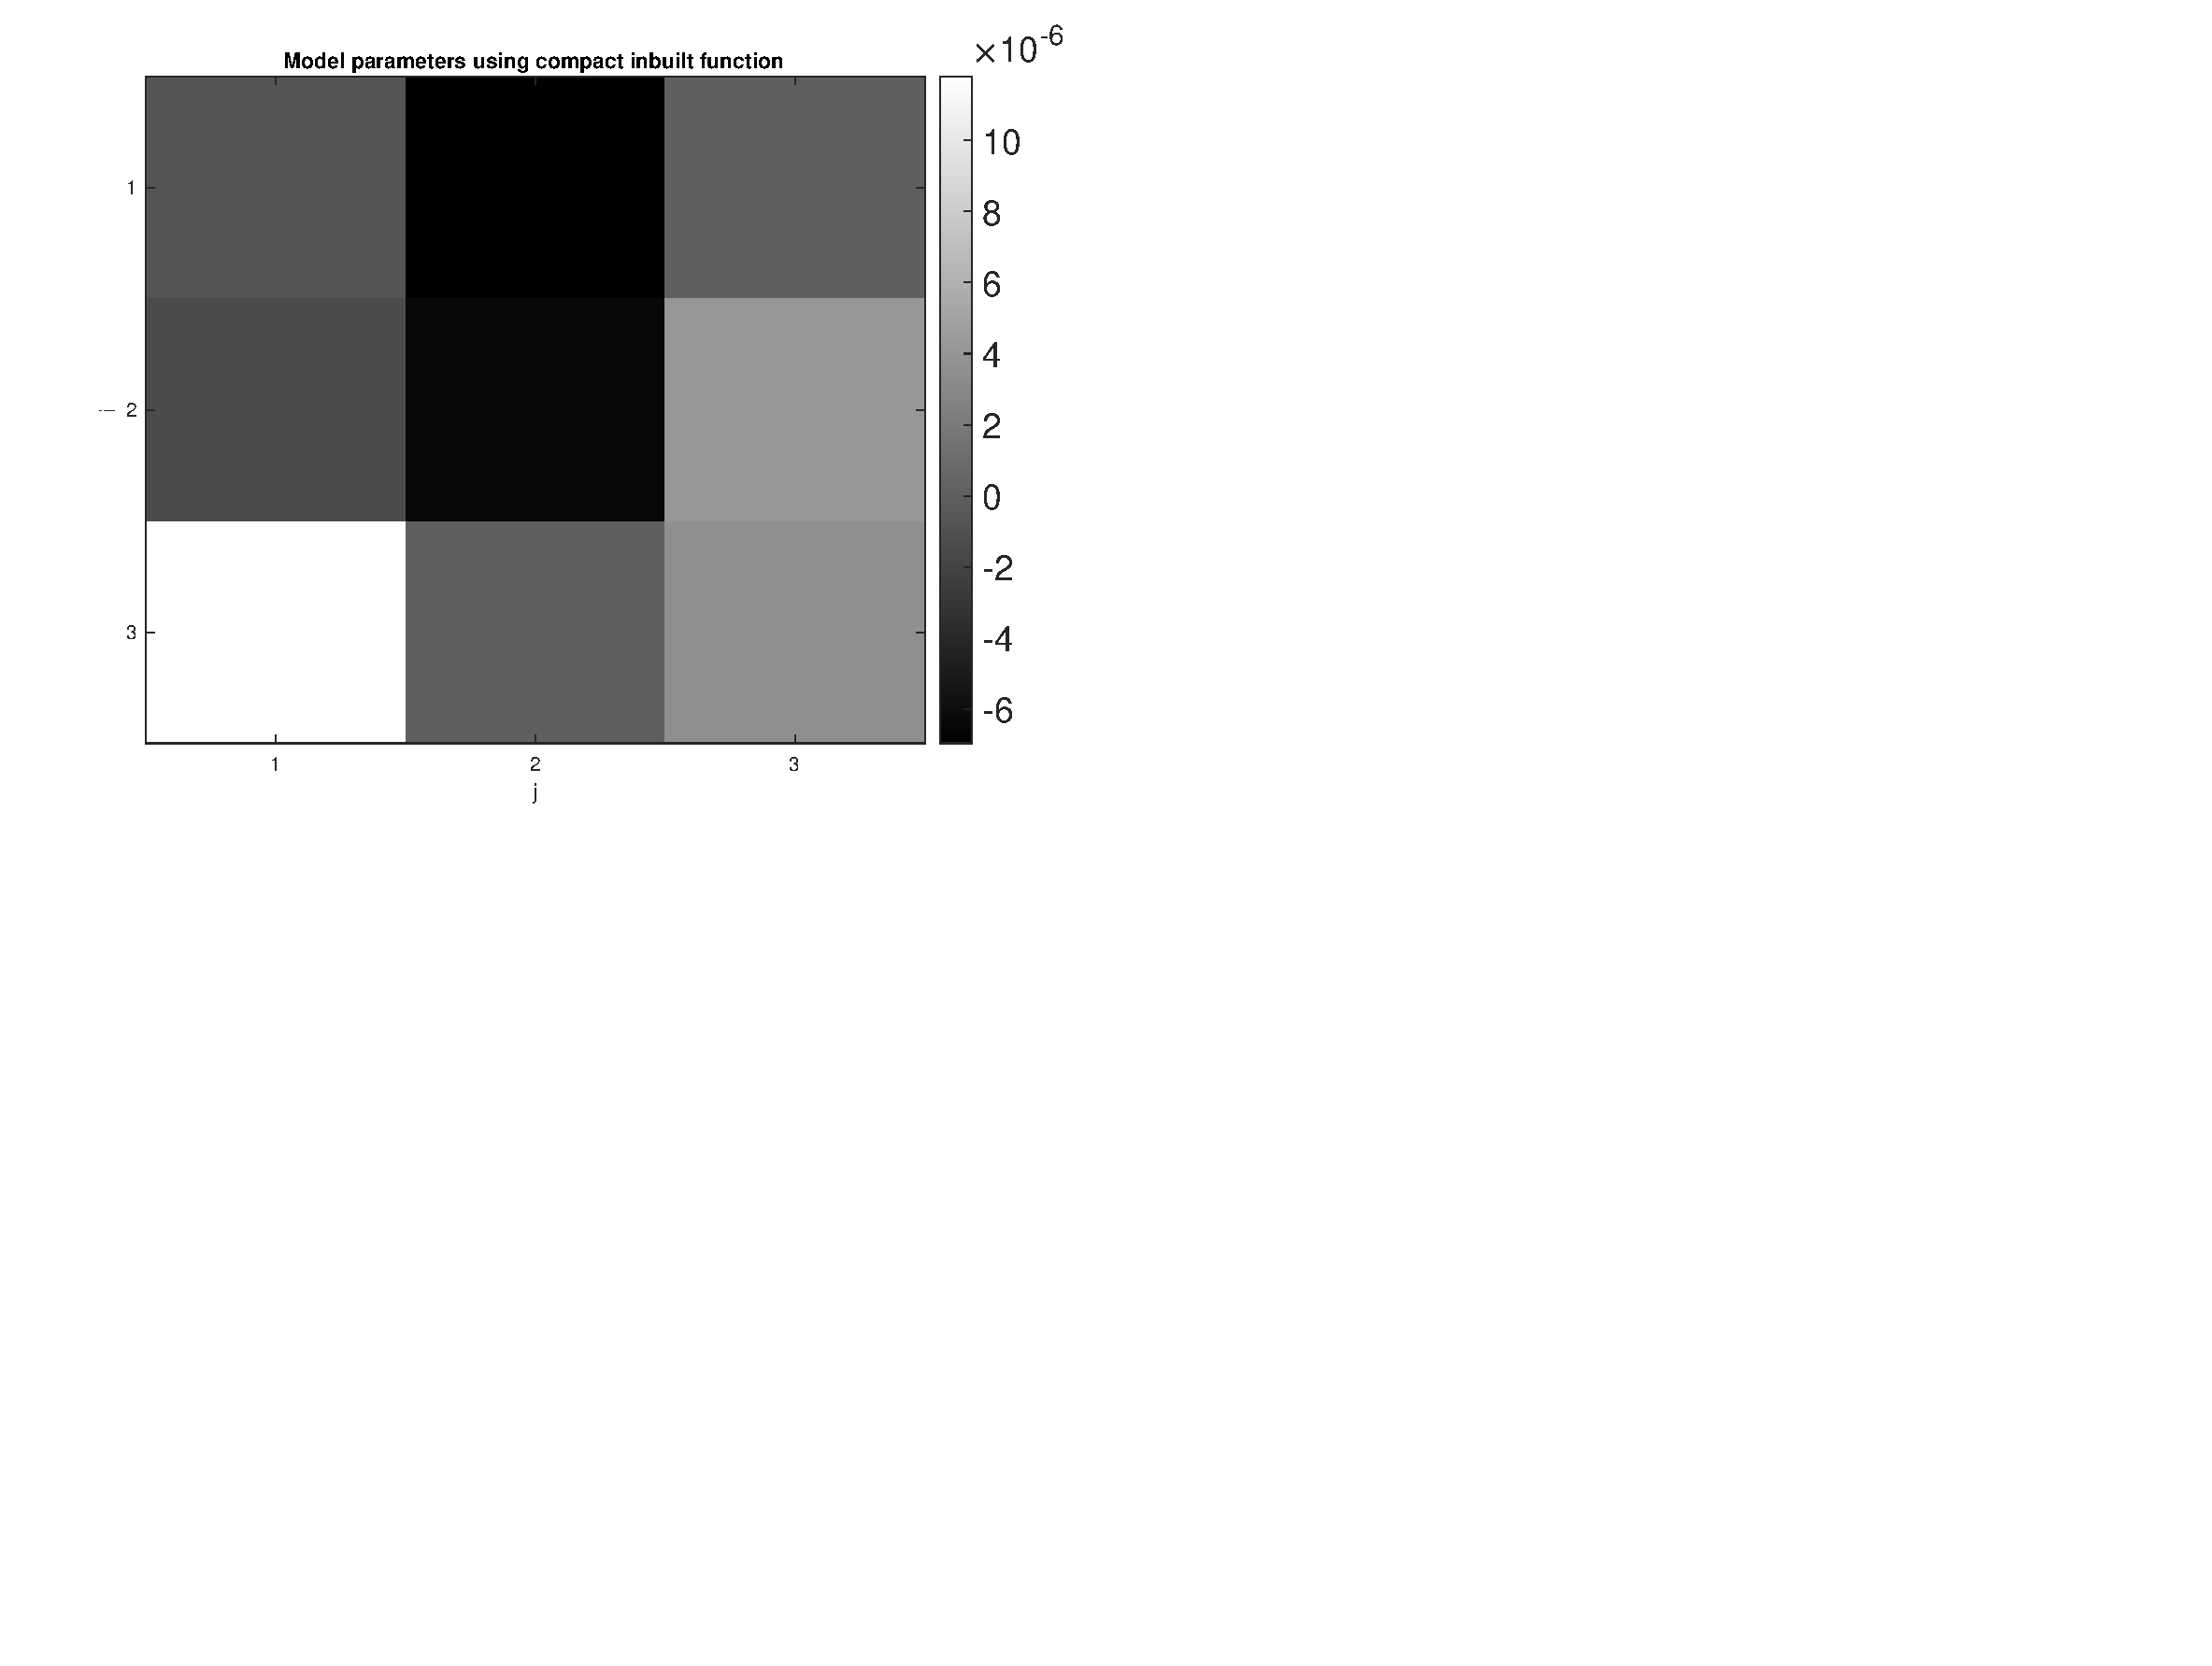
\includegraphics[width=\maxwidth{56.196688409433015em}]{figure_1.eps}
\end{center}
The values of the model parameters obtained in 3(a) (i) using the generalized inverse of $G$, with the compact SVD decomposition at positions; $ s_{12}$,  $s_{15}$, $s_{16}$, $ s_{17}$,   and  $s_{19}$, are smaller than their corresponding values obtained using the inbuilt function in 3(a)(ii). The remaining values of model parameters in 3(a)(i) are bigger than that in 3(a)(ii).\\

\begin{align*}
t_{dagger} = 10^{-4} \times
\begin{bmatrix}
     0.0967\\
   -0.1333\\
    0.0767\\
   -0.0767\\
   -0.0367\\
    0.1533\\
   -0.0500\\
    0.0500
 \end{bmatrix}~~~~~~~~~ t_{backslash} = 10^{-4} \times
\begin{bmatrix}
     0.0967\\
   -0.1333\\
    0.0767\\
   -0.0767\\
   -0.0367\\
    0.1533\\
   -0.0500\\
    0.0500
 \end{bmatrix}  ~~~~error = 10^{-5} \times
 \begin{bmatrix}
    -0.3667\\
   -0.3667\\
   -0.3667\\
    0.3667\\
    0.3667\\
    0.3667\\
    0.0000\\
   -0.0000\\
 \end{bmatrix}\end{align*}

The  predicted data sets obtained using model parameters in  3(a) (i) and 3(a) (ii) are the same and this is shown  by the figure below. The actual data however deviates from the predicted data by a value of -0.3667 for the first three data points, and 0.3667 the next three data  , and is the same for the last  two values.



\begin{center}
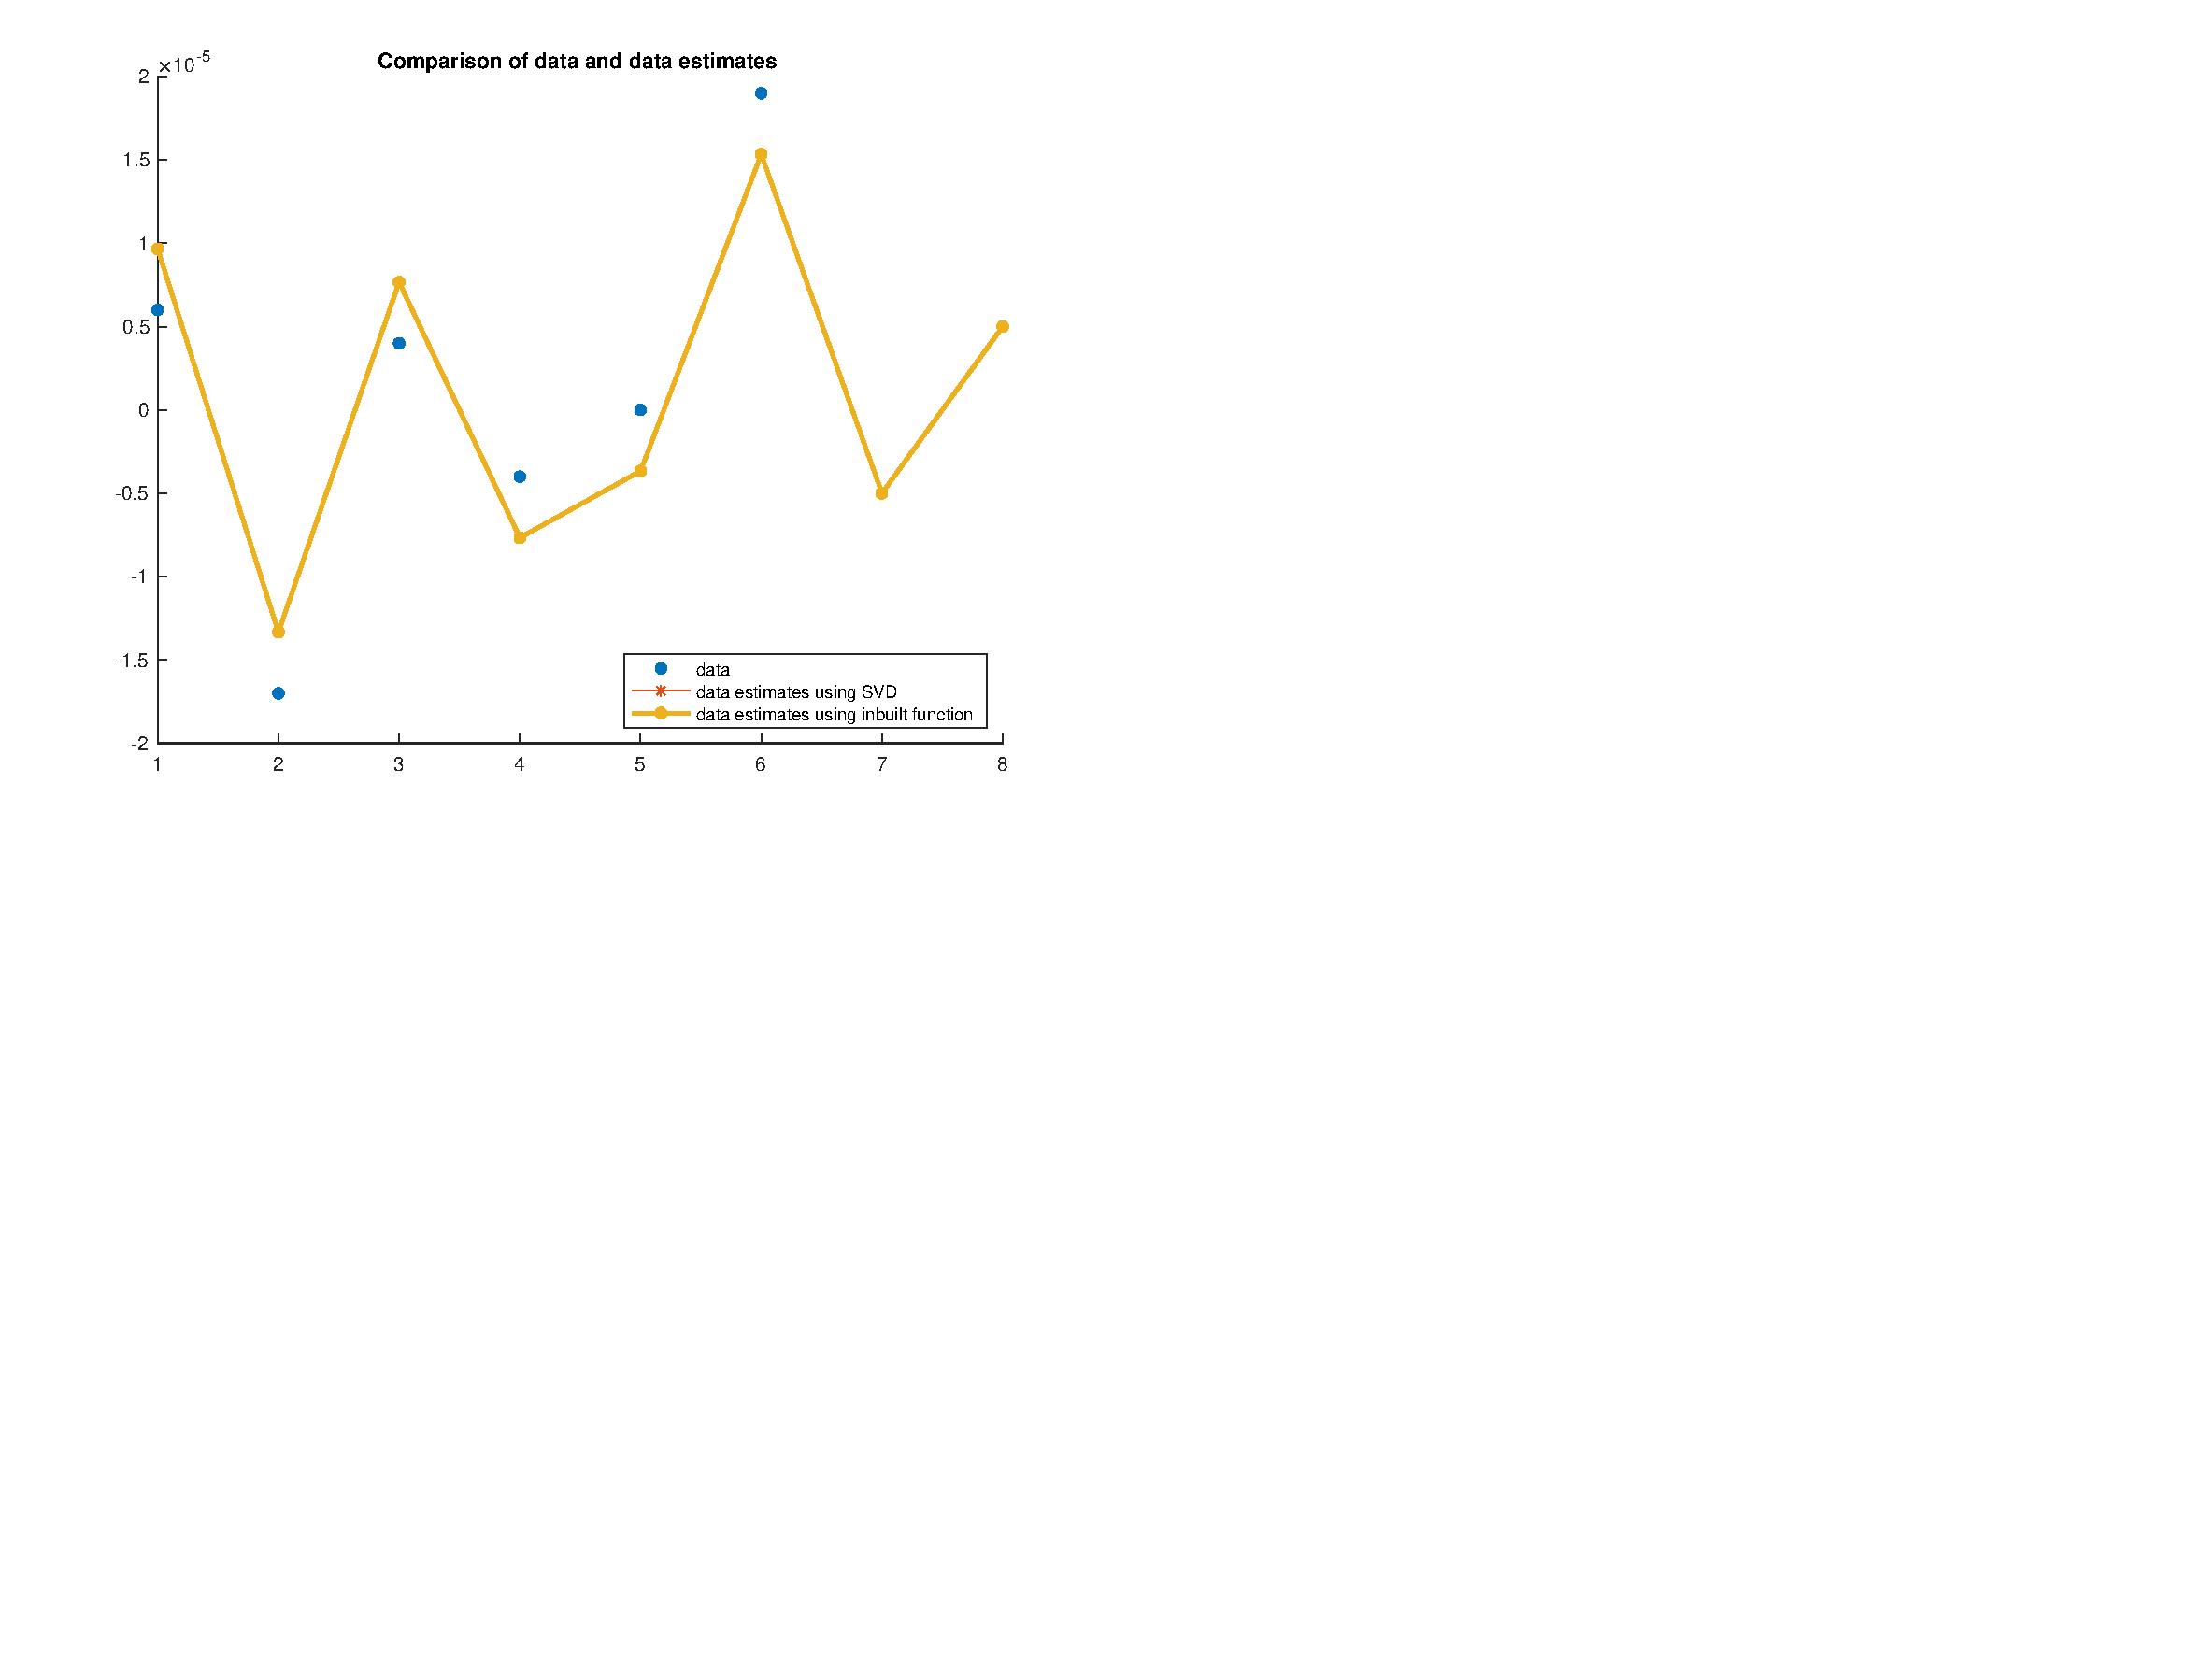
\includegraphics[width=\maxwidth{56.196688409433015em}]{figure_2.eps}
\end{center}

$\textbf{3(b)}$\\



dimesion of data null space= 1\\
The basis vector spanning the data null space is given by;\\
$\begin{bmatrix}
   0.4082\\
   0.4082\\
    0.4082\\
   -0.4082\\
   -0.4082
   -0.4082\\
  -0.0000\\
   -0.0000\\
\end{bmatrix}$

\begin{center}
\includegraphics[width=\maxwidth{56.196688409433015em}]{figure_3.eps}
\end{center}

$\textbf{3(c)}$\\

dimension of the model null space = 2\\
Therefore the model null space, $N(G)$, is spanned by the two orthonormal vectors that form the 8th and 9th columns of singular vector$V$. An orthonormal basis for the model null space is;\\
 $\begin{bmatrix}
  0.3357  &  0.2323\\
   0.2323  & -0.3357\\
   -0.5680   & 0.1035\\
 -0.2323   & 0.3357\\
 -0.3357  & -0.2323\\
    0.5680  & -0.1035\\
  -0.1035  & -0.5680\\
   0.1035    &0.5680\\
 -0.0000   & 0.0000\\
\end{bmatrix}$


\begin{center}
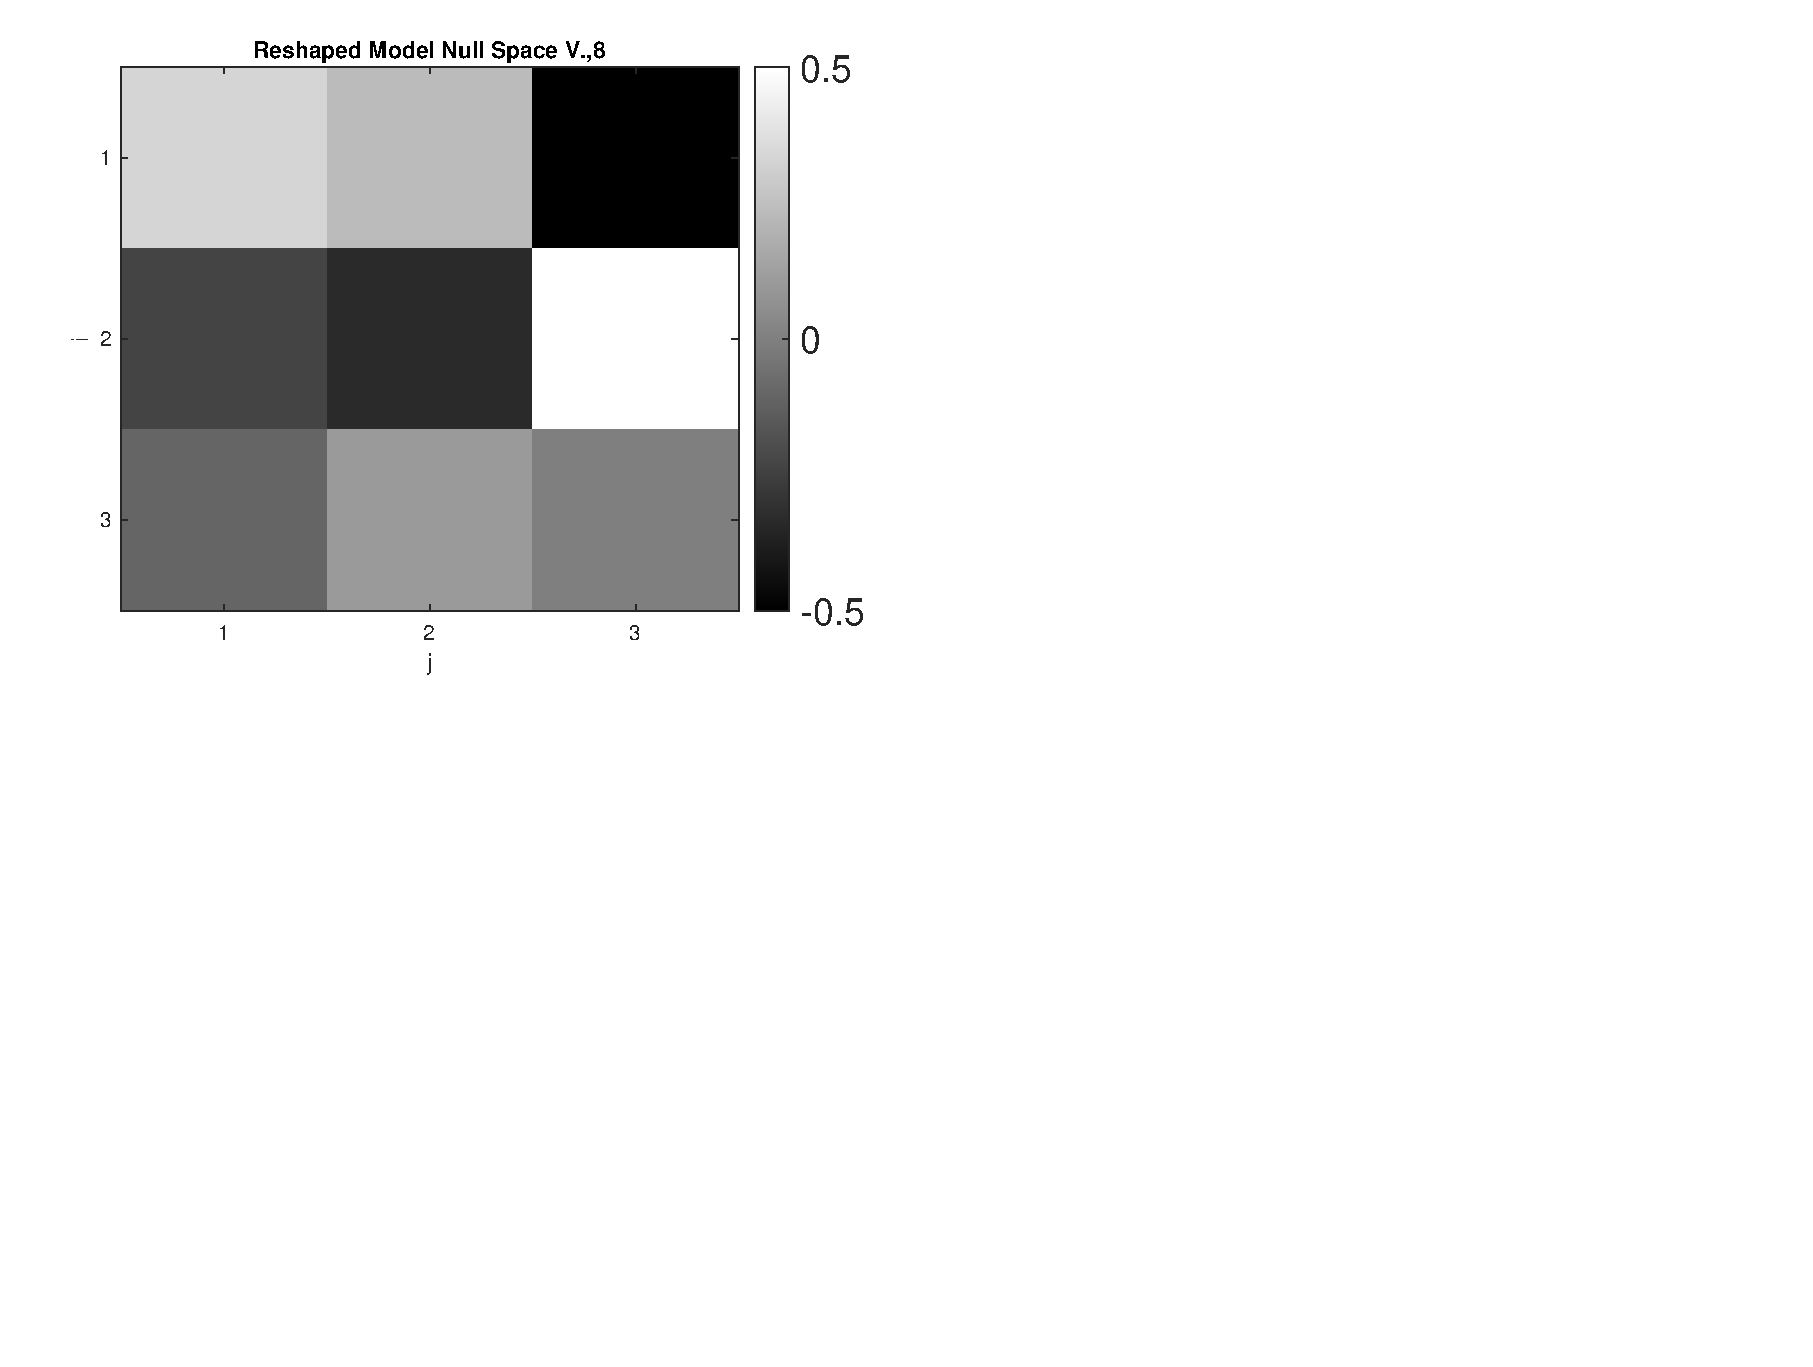
\includegraphics[width=\maxwidth{56.196688409433015em}]{figure_4.eps}
\end{center}



\begin{center}
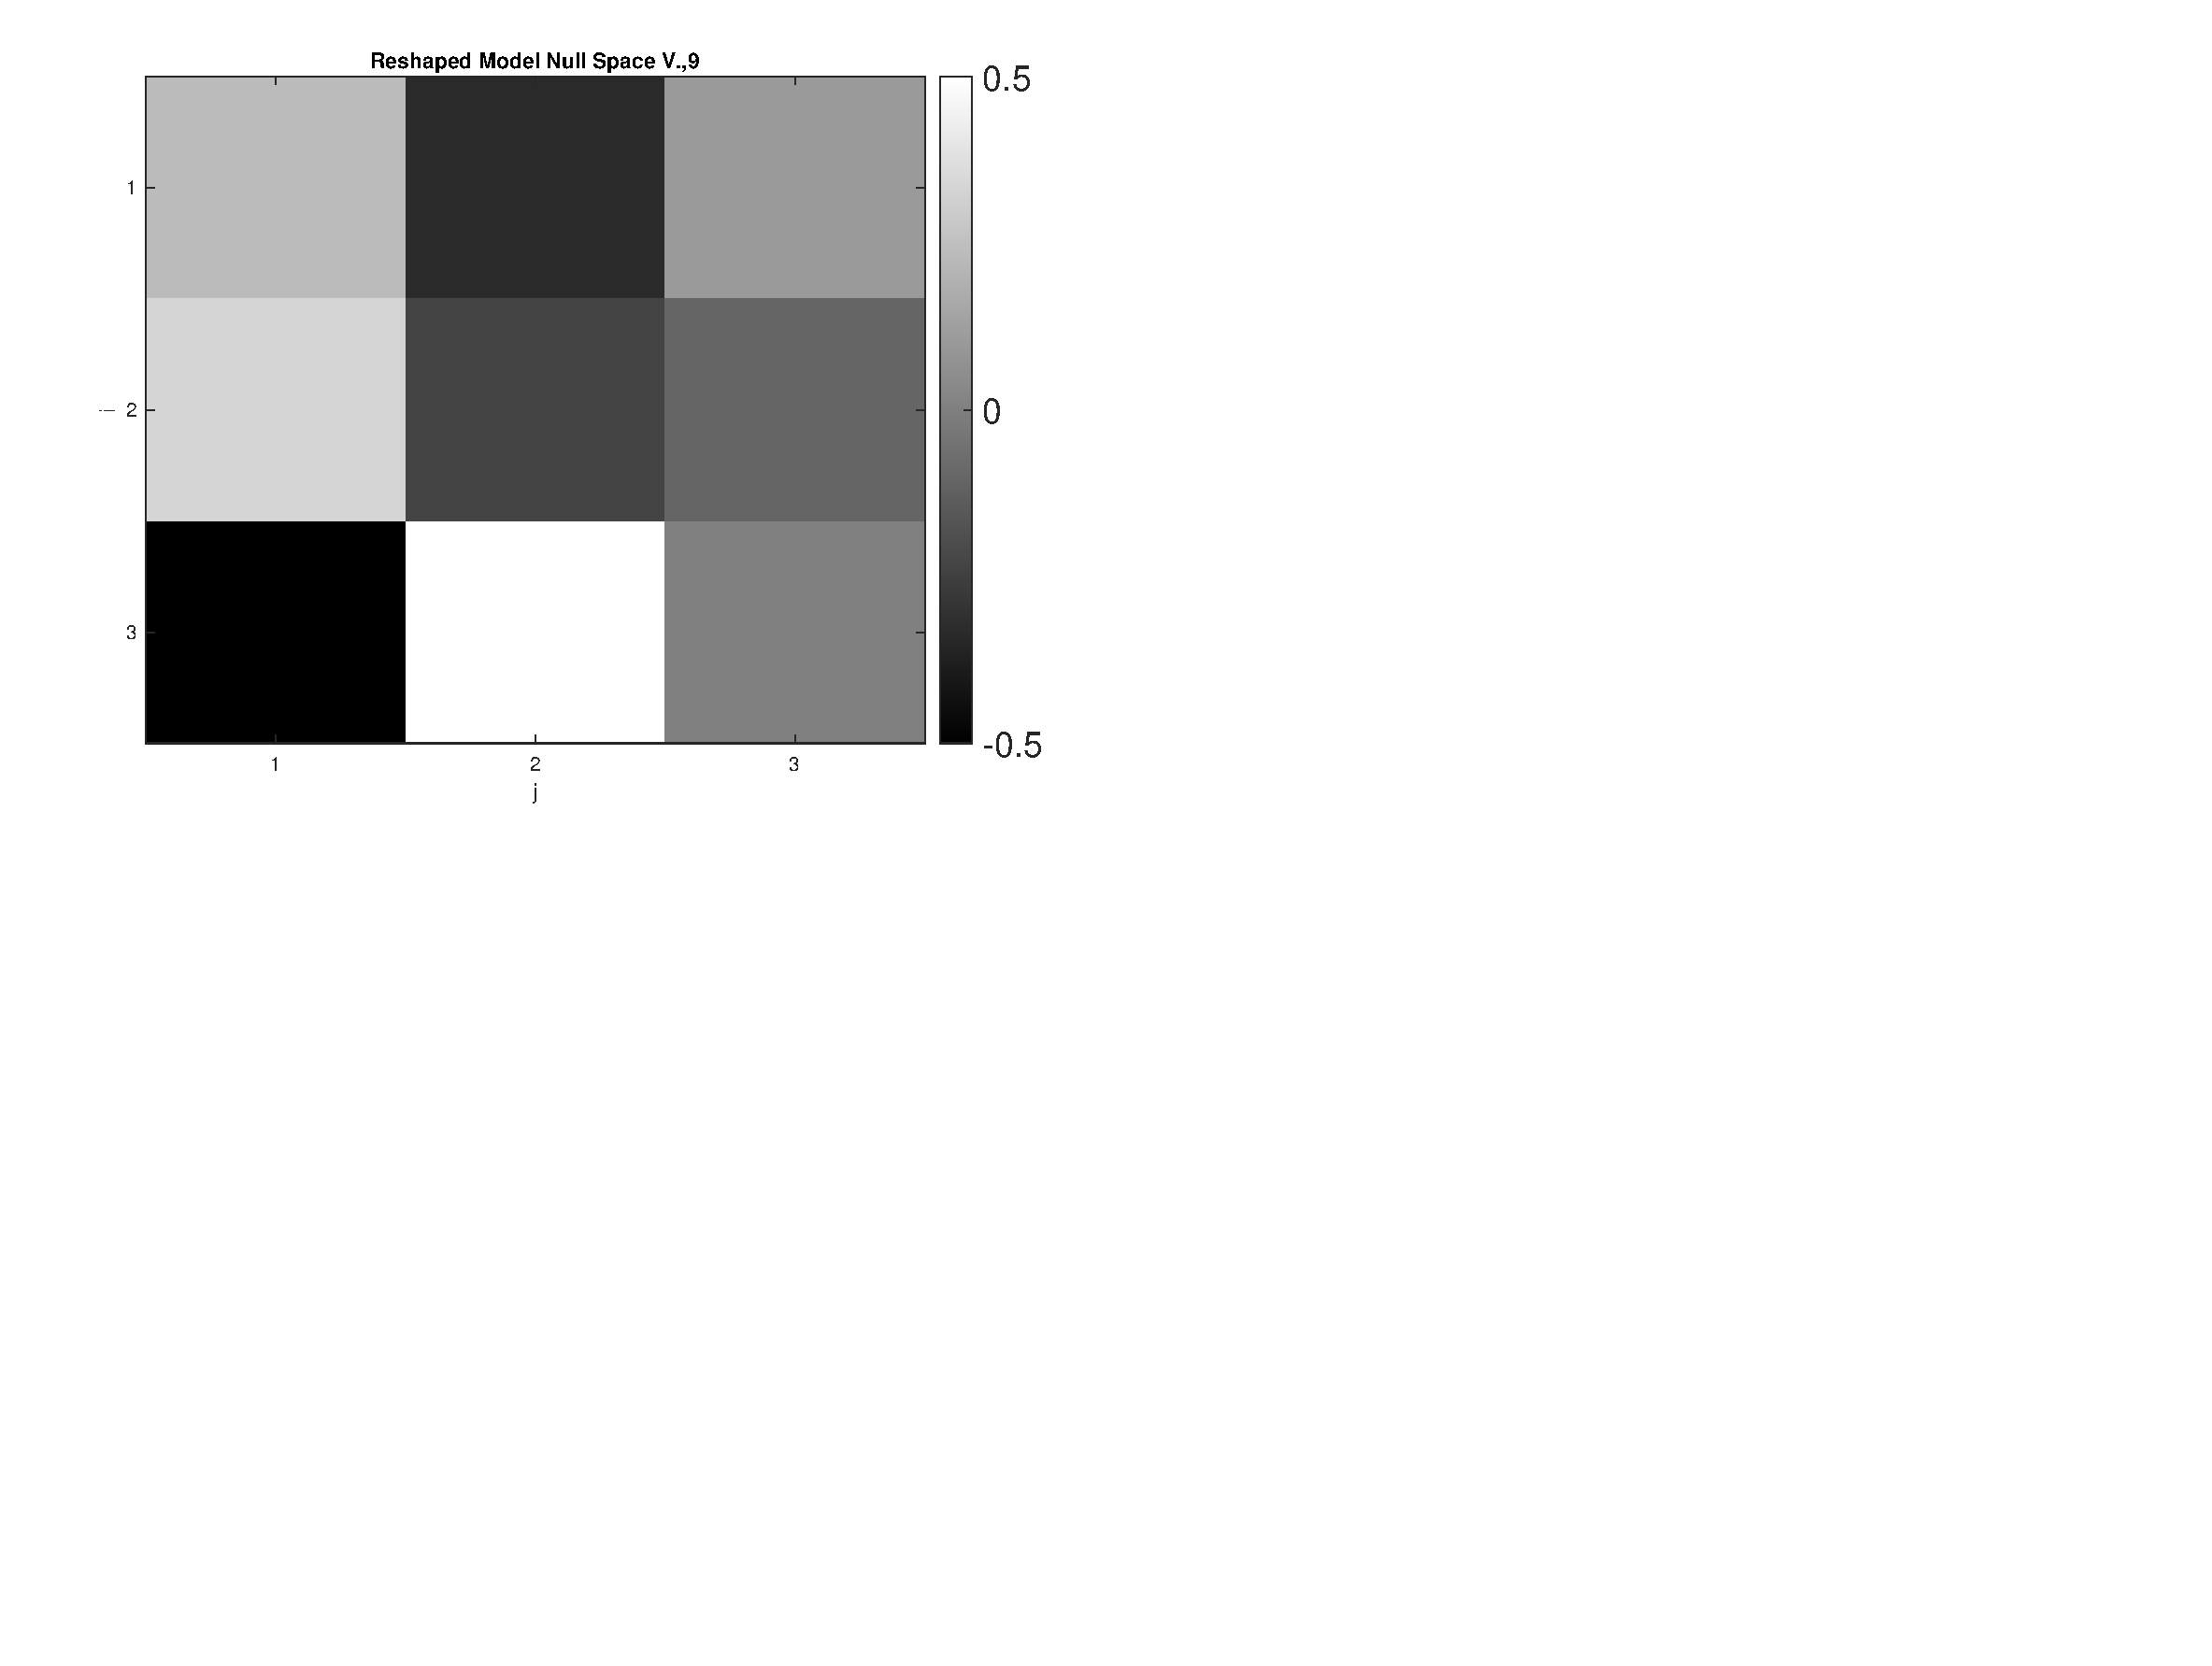
\includegraphics[width=\maxwidth{56.196688409433015em}]{figure_5.eps}
\end{center}


$\textbf{3(d)}$\\

Yes, it possible to have two sets of parameters that produce the same data. This is because the dimension of the model null space is two meaning that there are two non-zero vectors spanning the model null space and consquently we can always obtain new sets of model parameters that can give us the same data using;
$m = m_{\dagger} + \alpha _1V_8 + \alpha _2 V_9$  where  $V_8 $ and  $V_9$ span $N(G)$  and $ \alpha _1 , \alpha _2 \in \mathbb R $.\\

This can be seen in 3(a) above where the model paremeters obtained by generalized inverse of G, with the compact SVD decomposition different from the model parameters obtained using the backslash inbuilt function both give the same predicted data. Another set of parameters obtained using the expression above  gives the same data set as shown below.

If the basis of the model null space was to be empty, then there would be no two sets of parameters that would produce the same data.
 \begin{matlabcode}
new_m = mdagger + 2*V(:,8)+ 3*V(:,9);
d=G*new_m
\end{matlabcode}
\begin{matlaboutput}
d = 8x1    
1.0e+-4 *

    0.0967
   -0.1333
    0.0767
   -0.0767
   -0.0367
    0.1533
   -0.0500
    0.0500

\end{matlaboutput}

$\textbf{3(e)}$\\
Yes,it possible to have two sets of data that produce the same model parameters. This is because the dimension of the data null space is one meaning that there is one non-zero vector spanning the data null space and consquently we can always obtain a new data set  that can give us the same model parameters using;
$d = d_{\dagger} + \alpha _1 U_8 $  where  $U_8 $  spans $N(G^T)$  and $ \alpha _1 \in \mathbb R $.\\

An example to confirm this is as shown below where the new data gives the same set of parameters  as that obtained when using  the actual data set.
 
If the basis of the data null space was to be empty, then there would be no two data sets  that would give the same set of model parameters.

\begin{matlabcode}
new_d = d+ 10*U(:,8);
mdagger2 = Vp* inv(Sp)*Up.'*new_d
\end{matlabcode}
\begin{matlaboutput}
mdagger2 = 9x1    
1.0e+-5 *

   -0.0369
   -0.8697
    0.1399
    0.0303
   -0.6702
    0.2732
    0.9732
    0.2066
    0.3536

\end{matlaboutput}


$\textbf {APPENDIX}$

\begin{matlabcode}
t = [6e-06;-1.7e-05; 4e-06;-4e-06;0; 1.9e-05; -5e-06;5e-06];
s2=sqrt(2);
G = [1,0,0,1,0,0,1,0,0;
     0,1,0,0,1,0,0,1,0;
     0,0,1,0,0,1,0,0,1;
     1,1,1,0,0,0,0,0,0;
     0,0,0,1,1,1,0,0,0;
     0,0,0,0,0,0,1,1,1;
     s2,0,0,0,s2,0,0,0,s2;
     0,0,0,0,0,0,0,0,s2];

% Find dimensions of G
[m,n]=size(G);
% Get the singular values for the system matrix
[U,S,V] = svd(G);
 p=rank(G);


% Using the compact form
%Gdagger = pinv(G);
%mdagger = Gdagger*t
diag(S);
Vp = V(:,1:p);
Up =U(:,1:p);
Sp = S(1:p,1:p);

mdagger = Vp* inv(Sp)*Up.'*t


%Using backslash
mbackslash = G\t
tdagger = G*mdagger

tbackslash= G*mbackslash
error = t-tdagger
tt = linspace(1,8,8)

scatter(tt,t,'filled')
hold on
plot(tt,tdagger)
hold on 
plot(tt,tbackslash,'*','Color','black')
hold off
legend('data','data estimates using SVD','data estimates using inbuilt function','Location','eastoutside')
title('Comparison of data and data estimates')



%dimension of the data null space
m-p
U(:,p+1:m)

% Display image of null space model V.,9
%m0 = reshape(U(:,p+1),2,2)

plot(tt,U(:,p+1))
xlabel('j')

ylabel('i')
title('Data Null Space U.,8');
%dimension of the model null space
n-p

%model null space 
V(:,p+1:n)

% Display null space vectors reshaped to match tomography example geometry
m01=reshape(V(:,p+1),3,3)';

m02=reshape(V(:,p+2),3,3)';
% Display image of null space model V.,8
figure(1)
clf
colormap('gray')
imagesc(m01)
caxis([-0.5 0.5]);
set(colorbar,'Fontsize',18);
set(gca,'xtick',[1,2,3]);
set(gca,'ytick',[1,2,3]);
xlabel('j')
ylabel('i')
title('Reshaped Model Null Space V.,8');
% Display image of null space model V.,9
figure(2)
clf
colormap('gray')
imagesc(m02)
caxis([-0.5 0.5]);
set(colorbar,'Fontsize',18);
set(gca,'xtick',[1,2,3]);
set(gca,'ytick',[1,2,3]);
xlabel('j')
ylabel('i')
title('Reshaped Model Null Space V.,9');

\end{matlabcode}

\end{document}
